\documentclass[letterpaper,12pt,fleqn]{article}
\usepackage{matharticle}
\pagestyle{plain}
\begin{document}
\section*{Lab 5: The Cross Product}

Before we learn about relations and then functions, we need to add one more set operation
to our repertoire: the \emph{cross product}. Before defining the cross product, we need to
define what we mean by an \emph{ordered pair}. An ordered pair is exactly what it sounds
like: two numbers with a specific order. We represent ordered pairs like this:
\[(a,b)\]
The two numbers are in parenthesis and separated by a comma. In this case, $a$ comes
first, followed by $b$ --- the order is significant!

In order for two ordered pairs to be equal, both of their corresponding components must
be equal:
\[(a,b)=(c,d)\iff a=c\ \mbox{and}\ b=d\]
Note that $(a,b)$ is not equal to $(b,a)$ unless $a=b$. For example:
\begin{eqnarray*}
(1,3) &=& (1,3) \\
(1,3) &\ne& (3,1) \\
(1,3) &\ne& (1,2) \\
(1,3) &\ne& (2,3) \\
(1,1) &=& (1,1)
\end{eqnarray*}

Now, given two sets $A$ and $B$, we define their cross product as:
\[A\times B=\{(a,b)\mid a\in A\ \mbox{and}\ b\in B\}\]
Thus, we make a set of ordered pairs consisting of all possible elements from $A$
paired up with all possible elements of $B$.

When the sets are small and finite, it is easy to list out the elements of the cross
product. For example, when $A=\{1, 2, 3\}$ and $B=\{10, 20\}$:
\[A\times B=\{(1,10), (1,20), (2,10), (2,20), (3,10), (3,20)\}\]
Note that since $A$ has $3$ elements and $B$ has $2$ elements, $A\times B$ has
$3\cdot2=6$ elements.

Now you try. Let $A=\{1,2,3,4\}$ and $B=\{\pi,\sqrt{2}\}$:
\[A\times B=\]
Your cross product set should have $4\cdot2=8$ elements.

\newpage

When the sets involved are infinite, it is not possible to list all of the possible
elements; however, we should be able to recognize what the elements look like:

List $3$ possible elements of the set $\N\times\Q$:
\begin{enumerate}
\item
\item
\item
\end{enumerate}

And what about cross products of intervals? These will map out regions in the plane.
For example, $[-1,2]\times[-3,3]$ would be as follows:

\bigskip

\begin{minipage}{\textwidth}
  \centering
  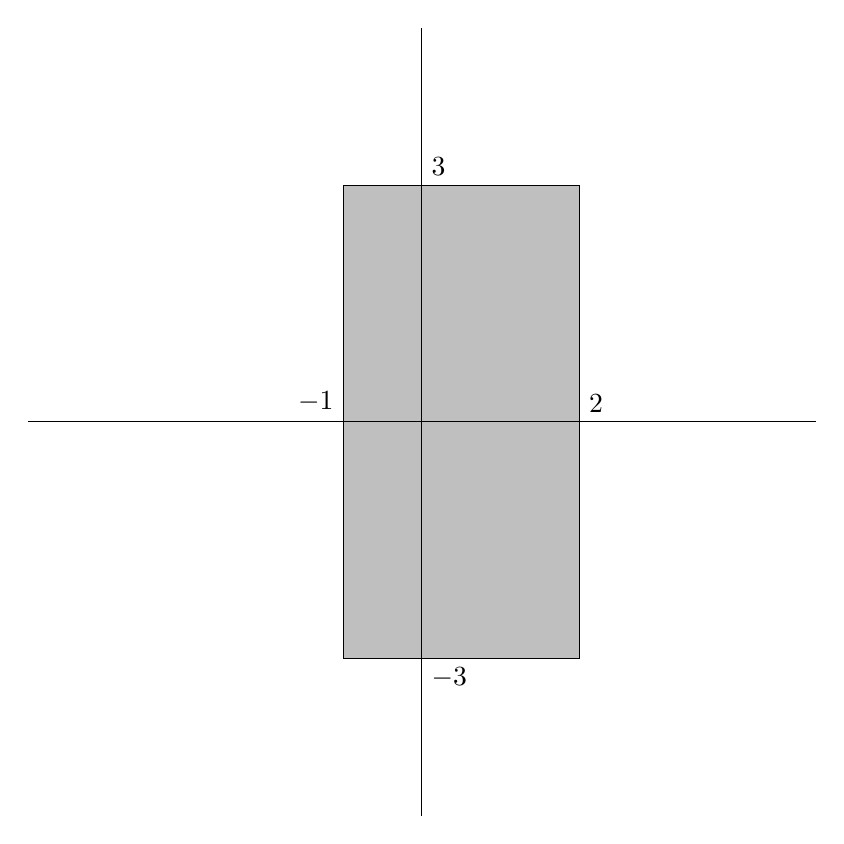
\begin{tikzpicture}
    \draw [fill=lightgray] (-1,-3) rectangle (2,3);
    \draw (-5,0) -- (5,0);
    \draw (0,-5) -- (0,5);
    \node [above left] at (-1,0) {$-1$};
    \node [above right] at (2,0) {$2$};
    \node [below right] at (0,-3) {$-3$};
    \node [above right] at (0,3) {$3$};
  \end{tikzpicture}
\end{minipage}

Here we overlay the first interval along the $x$-axis and the second interval along the
$y$-axis. Note that every point within the filled rectangle defined by these intervals
represents an element in the cross product of the intervals. For example: $(0,0)$ is
an element of the cross product; however $(3,1)$ is not.

If $A=[-1,2]$ and $B=[-3,3]$ as above, determine whether each of the following points
is or is not in $A\times B$. Be sure to use `$\in$' and `$\notin$' to indicate your
choice:
\begin{enumerate}
\item $(1,1)\quad A\times B$
\item $(-2,0)\quad A\times B$
\item $(-1,-3)\quad A\times B$
\item $(3,3)\quad A\times B$
\end{enumerate}

The cross product does not have to be a contiguous, continuous region. The following
problem demonstrates this:

Let:
\[A=[-1,2]\cup[3,4]\]
\[B=[-3,2]\]
Draw $A\times B$ below:

\bigskip

\begin{minipage}{\textwidth}
  \centering
  \begin{tikzpicture}
    \draw (-5,0) -- (5,0);
    \draw (0,-5) -- (0,5);
  \end{tikzpicture}
\end{minipage}

\bigskip

Indicate whether the following points are in or not in $A\times B$:
\begin{enumerate}
\item $(-2,2)\quad A\times B$
\item $(0,0)\quad A\times B$
\item $(\frac{5}{2},1)\quad A\times B$
\item $(3,2)\quad A\times B$
\end{enumerate}

\end{document}
